\chapter{Physics Background}
\label{chap_phys}

\section{$J/\psi$ production process}
$J/\psi$ was discovered in $p$+Be$\rightarrow$$e^{+}e^{-}X$ at AGS and $e^{+}e^{-}$ annihilation at SPEAR in Stanford Linear Accelerator Center (SLAC) in 1974~\cite{bib_jpsifirst1,bib_jpsifirst2}.
$J/\psi$ is a resonance state of $c\bar{c}$ and $J/\psi$ mass is 3096.9 MeV/$c^{2}$ slightly higher than the charm quark pair mass. 
$J/\psi$ has spin=1 without the orbital angler momentum.   

Production of $J/\psi$ can be classified into two processes, where the first process is the creation of $c\bar{c}$ and the second one is to form $J/\psi$ from $c\bar{c}$ pairs.
Since the mass of charm quarks is expected large enough compared to $\Lambda_{QCD}\sim$ 200 MeV, $c\bar{c}$ production can be described by the pertubative QCD calculation. 

\begin{figure}[!h]
  \centering
  \includegraphics[width=12cm]{chap2/figure/ccbar_diagram.png}
  \caption{Feynman diagrams of $c\bar{c}$ production. From left to right, they express gluon fusion, gluon splitting, and flavor excitation, respectively. }
  \label{fig_2_jpsidiagram}
\end{figure}

\begin{figure}[!h]
  \centering
  \includegraphics[width=8cm]{chap2/figure/production/ccbar.png}
  \caption{
    Total cross section of $c\bar{c}$ in pp collisions as a function of $\sqrt{s}$.  
    The contribution from pair creation, flavor excitation, and gluon splitting are shown separately~\cite{bib_ccbar}.
  }  
  \label{fig_2_charmxsection}
\end{figure}
Figure~\ref{fig_2_jpsidiagram} shows the Feynman diagrams of the main $c\bar{c}$ production at LHC energies~\cite{bib_ccbar}. 
The leading order of $c\bar{c}$ production is gluon fusion.
In this process, gluons from each nucleus interact and produce $c\bar{c}$. 
The next-leading order process is the gluon splitting, which scattered gluons split into $c\bar{c}$ pairs.
Another next-leading order process is flavor excitation, where a off-shell quarks produced by the virtual gluon splitting is scattered with a gluon in the other nucleus. 
Figure~\ref{fig_2_charmxsection} shows the calculated cross section of $c\bar{c}$ production and the contribution of each process in pp collisions as a function of the collision energy~\cite{bib_ccbar}. 

Several models have been developed to describe $J/\psi$ formation from $c\bar{c}$ pairs such as the color singlet model (CSM), color evaporation model (CEM), and Non-Relativistic QCD (NRQCD)~\cite{bib_csm1,bib_csm2,bib_cem1,bib_cem2}. 
However, for the moment, no model describes $J/\psi$ production and polarization simultaneously. 

%\subsubsection{Color Singlet Model (CSM)}
%The color singlet model (CSM) is assumed that a specific qaurkonium state can be formed if the charm quark anti-charm quark pairs created color singlet state with the same angler momentum quantum number as $J/\psi$. 
%In this model, hard gluon emission is needed to conserve C-parity. 

%In the leading order gluon fusion process, $J/\psi$ production whose spin number is 1 is suppressed compared to other quarkonia with spin 0 or 2 because gluons have spin 1.

%\subsubsection{color Evaporation Model (CEM)}
%In this model, the probability of $J/\psi$ formation is independent the color of $c\bar{c}$ pairs. 
%The color of $c\bar{c}$ is assumed to be neutralized by the interaction with collision induced color field. 

%\subsection{Non-Relativistic QCD (NRQCD)}
%The charmonium can be produced in a color singlet or color octet.
%the spin can be singlet or triplet and it can also have orbital angular momentum.

%\subsection{Feed Down $J/\psi$}
%CMS


\section{$J/\psi$ production in Relativistic Heavy Ion Collisions}
\label{sec_2_summary}
Compared to pp collisions, $J/\psi$ undergoes the following effects in heavy ion collisions. 
\begin{description}
  \item[Color screening]\mbox{} \\
	$J/\psi$ is not formed in QGP since attraction between charm and anti-charm quarks are screened in QGP as described in Section.~\ref{sec_2_screening}
  \item[Regeneration in QGP]\mbox{} \\
		Since the number of $c\bar{c}$ at the RHIC and LHC energies are large in heavy ion collisions, $J/\psi$ can be formed in the QGP or phase boundary from uncorrelated $c\bar{c}$ (each of pairs is produced in different nucleon-nucleon collisions.)
  \item [Modification of gluon PDF in nuclei]
	It is known as the gluon yield in nuclei is smaller than those in free proton scaled by the atomic number. 
	This is called  as the gluon shadowing. Since gluon parton distribution function (PDF) in nuclei is different from gluon PDF in free proton, simple A scaling of $J/\psi$ production from pp collisions to heavy ion collisions is not preserved.
  \item [Cronin effect]
	It is known	the momentum spectra in p-$A$ collisions become harder compared with pp collisions. 
	This is called as Cronin effect. 
	The harder shape of the transverse momentum $p_{\rm{T}}$ is expected due to the multiple scattering of incident partons in the nucleus. 
   \item [Break up and energy loss in nuclei]
%  \item [Nuclear absorption]
	$J/\psi$ or pre-resonance $c\bar{c}$ state are destructed by the collisions with spectator nucleons, which leads to the suppression of the $J/\psi$ production. 
	This depends on the relative time scale of $c\bar{c}$ of $J/\psi$ formation and crossing time of two colliding nuclei. 
	The medium induced radiative parton energy loss is expected  and depends on their formation time. 
	If the formation time of gluon emission is larger than the nuclear mean free path, this is expected coherent process. 
\end{description}
Color screening is explained in Section.~\ref{sec_2_screening}.
$J/\psi$ regeneration is described in Section.~\ref{sec_2_reco}.
The normal nuclear matter effects are summarized in Section.~\ref{sec_2_normal}.

\section{Color Screening in QGP and suppression of $J/\psi$}
\label{sec_2_screening}
Matsui and Satz proposed the suppression of $J/\psi$ production as one of the strong evidence of the QGP formation\cite{bib_matsui}. 
The mechanism is based on the Debye screening observed in the electromagnetic plasma. 
At zero temperature, the QCD potential between the quark and anti-quark is expressed by, 
\begin{equation}
V_{QCD}(r) = -\frac{4}{3}\frac{\alpha_{s}(r)}{r}+\sigma r
\label{eq_2_jpsiv}
\end{equation}
where $r$ is the distance between the quark and anti-quark and $\sigma$ is the QCD string tension. 
$\alpha_{s}$ is the gauge coupling constant of QCD described in Section~\ref{sec_1_qcd}. 

Figure~\ref{fig_2_freeenergy} shows the free energy of color singlet quark anti-quark pairs(F(r, T)) calculated by (2+1) lattice QCD~\cite{bib_jpsimodel}.  
The asymptotic value (F($\infty$, T)) corresponding to the energy needed to separate the quark anti-quark pair decrease with increasing temperature. 
\begin{figure}[!h]
  \centering
  \includegraphics[width=10cm]{chap2/figure/Suppression/FreeEnergy.png}
  \caption{Color singlet quark-antiquark free energy as a function of quark separation calculated in (2+1) lattice QCD at different temperature~\cite{bib_jpsimodel}.}
  \label{fig_2_freeenergy}
\end{figure}
%If the $\lambda_{D}$ becomes smaller than the hadronic radius, quark-antiquark pairs cannot interact with each other and become unbound. 


As the temperature increases, many free colored partons are generated and occupy the vacuum. 
The potential of the quark anti-quark pairs is modified from coulomb like potential to Yukawa potential, 
\begin{equation}
  V_{QCD}(r) = -\frac{4}{3}\frac{\alpha_{s}}{r}e^{-\frac{r}{\lambda_{D}(T)}}
\end{equation}
where $\lambda_{D}(T)$ is the debye length of the color screening. 
Qualitatively $\lambda_{D}(T)$ becomes smaller as temperature increases. 
According to lattice calculation, the second term of Eq.~\ref{eq_2_jpsiv} becomes small as temperature increases as following dependence~\cite{bib_tension}, 
\begin{equation}
  \sigma/\sigma_{0} = \sqrt{1-\frac{T}{T_{c}}}
\end{equation}
where $\sigma_{0}$ is the string tension at $T$$=$0.
At deconfined phase, second term in Eq.~\ref{eq_2_jpsiv} should be vanished or negligible small. 

Lattice calculations and potential models have been adopted to expect the dissociation temperature of each quarkonium. 
Due to the different binding energy, dissociation of quarkonium occurs sequentially towards high temperature. 
Table~\ref{table_2_melt} shows the summary of dissociation temperature $T_{d}$ in unit of $T_{c}$ for each quarkonium calculated by a potential model calculation~\cite{bib_melt}.

\begin{table}[!h]
  \centering
  \begin{tabular}{ccccccccc} \\ \hline
    State   & $J/\psi$  & $\chi_{c}(1P)$  & $\psi (2S)$ & $\Upsilon (1S)$ & $\chi _{b}(1P)$ & $\Upsilon (2S)$  & $\chi_{b}(2P)$  & $\Upsilon (3S)$ \\ \hline
    $T_{d}/T_{c}$ & 2.1 & 1.16 & 1.12 & $\geq 4.0$ & 1.76 & 1.60 & 1.19 & 1.17 \\ \hline
  \end{tabular}
  \caption{Dissociation temperature in unit of $T_{c}$ calculated using a potential model\cite{bib_melt}.  }
  \label{table_2_melt}
\end{table}

\section{$J/\psi$ Regeneration}
\label{sec_2_reco}
%The enhancement of baryon/meson ratio $\sim$ 1 is observed at in the intermediate $p_{T}\sim$ 3 GeV/c at RHIC\cite{bib_baryonmesonphenix}. 
%This cannot be described via fragmentation process but it can be described by the coalescence of neighboring quarks. 
%If the phase space is fulfilled by the quarks, the coalescence happens and generated hadrons carry the momentum of mother quarks.
\begin{figure}[!h]
  \centering
  \includegraphics[width=10cm]{chap2/figure/reco/jpsirege_schematics.png}
  \caption{
  	Schematics of $J/\psi$ regeneration in heavy ion collisions at RHIC and LHC~\cite{bib_regenature}.
	}
  \label{fig_2_recosche}
\end{figure}

The expected number of $c\bar{c}$ quarks created in heavy-ion collisions at the LHC, RHIC and SPS is about 60, 10, 0.2 as shown in Table~\ref{table_2_ncchic}, respectively.
\begin{table}
	\centering
	\begin{tabular}{cccc} \hline
	Experiment      &  SPS &  RHIC  & LHC  \\ \hline
	$N_{cc}$/$N_{ev}$ & 0.2   & 10 & 60 \\ \hline
	$dN_{ch}/d\eta$  & 450   &  650& 1500 \\ \hline	
	\end{tabular}
	\caption{Expected the number of $c\bar{c}$ and charged particles in central heavy ion collision at SPS, RHIC, and LHC. }
	\label{table_2_ncchic}
\end{table}
The yield of charmonium from regeneration depends on the ratio of the number of light quarks and charm quarks. 
The estimated number of regenerated $J/\psi$ is scaled by ($N_{coll}^{2}/N_{part}$).
%The number of $c\bar{c}$ pair production in nucleus-nucleus depends on the number of binary collisions ($N_{coll}$).
%On the other hand, light quark hadron yields are approximately scaled by the number of participants in the overlap region of colliding nuclei. 
%In the glauber calculation, $N_{coll}$ grows rapidly compared to the $N_{part}$ as the centrality of collisions increases. 
%Therefore the enhancement is more significant at central heavy ion collisions than peripheral collisions.  
Production of $c\bar{c}$ as a function of impact parameter (collision centrality) and the production of light hadrons 
scale with the number of binary collisions ($N_{coll}$) and the latter with the number of participants ($N_{part}$), respectively. 
Participants are defined as the nucleons which exist in the overlap area of colliding nuclei. 
The detail of the collision geometry of high energy nucleus-nucleus collisions is summarized in Appendix~\ref{app_a_glauber}.
Since $N_{coll}$ grows faster than $N_{part}$ as a function of centrality, regeneration of $J/\psi$ is more pronounced in more central collisions. 
The regeneration of $J/\psi$ is direct evidence of the formation of deconfied matter. 
At the LHC, where abundant $c\bar{c}$ are created, $J/\psi$ is possibly formed by the regeneration process from uncorrelated $c\bar{c}$ pairs, where $c$ and $\bar{c}$ are created in different nucleon-nucleon collisions since charm quarks are expected to be thermalized in QGP. 

Figure~\ref{fig_2_reco} shows the numerical calculation of $dN_{J/\psi}/dy$ as a function of $N_{part}$~\cite{bib_yellowpaper}.
The rapid increase with centrality shows due to the quadratic dependence of the number of $c\bar{c}$. 
%Figure~\ref{fig_2_reco} shows the transport model calculation in Pb-Pb collision at LHC at forward rapidity~\cite{bib_transport}. 
%The transport mode considers all both of QGP effects and normal nuclear matter effects. 
%According to this model calculation,  the contribution of $J/\psi$ regeneration is dominant below $p_{\rm{T}}~ <$ 4 GeV/$c$.
\begin{figure}[!h]
  \centering
  \includegraphics[width=10cm]{chap2/figure/reco/recoestimate.png}
  \caption{
	Calculation of regeneration model for $J/\psi$ production as a function of $N_{part}$ at LHC in three $c\bar{c}$ multiplicities~\cite{bib_yellowpaper}. 
	}
  \label{fig_2_reco}
\end{figure}

\section{Normal Nuclear Matter Effects in Relativistic Heavy Ion Collisions}
\label{sec_2_normal}

\subsection{Modification of Parton Distribution Function inside Nuclei}
\label{sec_2_pdf}
The cross section of the hard process between nucleon A and nucleon B is factorized as, 
\begin{equation}
  \sigma_{AB} =  \Sigma_{a, b} \int{dx_{1}}\int{dx_{2}} f^{A}(x_{1})f^{B}(x_{2})\sigma(a_{1}+b_{2})
\end{equation}
where $f^{A}$ and $f^{B}$ are the  parton distribution function (PDF). 
$\sigma(a_{1}+b_{2})$ is the cross section of partonic subprocess between the partons in A and B.
$x$ is a longitudinal momentum fraction of partons. 
In 2$\rightarrow$1 process, the relation of $x$,  rapidity, and energy is expressed by 
\begin{equation}
  x_{1, 2} = \frac{m_{T}}{\sqrt{s}}e^{\pm y}
\end{equation}
In 2$\rightarrow$2 process, the relation of x,  rapidity, and energy is expressed by 
\begin{equation}
%  x_{1, 2} = \frac{m_{T}}{\sqrt{s}}e^{\pm y}
  x_{1} = \frac{m_{T}}{\sqrt{s}}(e^{y_{1}}+e^{y_{2}}),  \\
 ~~~  x_{2} = \frac{m_{T}}{\sqrt{s}}(e^{-y_{1}}+e^{-y_{2}}) \\
\end{equation}
where $m_{T}$ is the transverse mass $m_{T}=\sqrt{m^{2}+p_{T}^{2}}$ and $\sqrt{s}$ is the collision energy per nucleon-nucleon collision in the center-of-mass system.
%In order to understand the experimental data,  the determination of PDF is crucial. 
%The useful way to determine the PDF is the Deep Inelastic Scattering (DIS)
PDF is mainly obtained from the results of deep inelastic scattering (DIS) and the calculated cross section using perturbative QCD as a function of $x$ and momentum transfer $Q^{2}$~\cite{bib_dis}. 
\begin{figure}[!h]
  \centering
  \includegraphics[width=10cm]{chap2/figure/CNM/hera.png}
  \caption{Parton distribution function measured via e-p scattering in H1 and ZEUS at HERA ~\cite{bib_hera}.}
  \label{fig_2_protonpdf}
\end{figure}
Figure~\ref{fig_2_protonpdf} shows the measured parton distribution function in protons via e-p scattering in H1 and ZEUS at HERA~\cite{bib_hera}.
They observed the rapid growth of the gluon PDF toward small $x$. 
This multiple gluon production at small $x$ is caused by long life time of the energy fluctuation and described by the BFKL equation ~\cite{bib_bfkl}. 
When the gluon density is not too high, gluons don't interact with each other and the linear growth remains. 
%%and the growth of gluon is expressed $\sim x^{-\lambda}$ with $\lambda$$\sim$0.3 by the linear BFKL equation~\cite{bib_bfkl}.
The life time of the gluon radiation with small fraction $x$ and transverse momentum transfer $k_{T}$ is, 
\begin{equation}
	\tau  \sim  \frac{1}{\Delta E} \sim \frac{2xp}{k_{T}}
\end{equation}
where $p$ is the mother parton momentum. 
Therefore this fluctuation has long life time at high energy limit and emitted gluon can generate gluons by $g\rightarrow gg$ with the probability of gluon emission$\sim~\alpha_{s}ln(1/x)$. 
Incoherent gluon emissions from gluons created in the previous steps can also occur and gluon density rapidly increase. 
In high energy pp or nucleus-nucleus collisions, scatterings of these small $x$ partons mainly occur. 

European Muon Collaboration (EMC) group observed the modification of nuclear parton distribution function (nPDF) compared to PDF in the free proton in $\mu$-Fe scattering in 1982 as shown in Fig.~\ref{fig_2_stfunc}~\cite{bib_emc}. 
The modification of the nPDF from the free proton is evaluated as the ratio of the structure function. 
They discovered the clear modification of the nucler modification factors for heavy ions. 
The right panel of Fig.~\ref{fig_2_stfunc} shows the ratio of the structure function in heavy nuclei and carbon. 
The suppression of $F^{A}_{2}/F^{C}_{2}$ is seen toward smaller $x$. 
%\begin{figure}[!h]
%  \centering
%  \includegraphics[width=8cm]{chap2/figure/CNM/emc.png}
%  \caption{The ratio of the nucleon structure functions F measured iron and deuterium as a function of $x$ measured by EMC collaboration~\cite{bib_emc}.}
%  \label{fig_2_emc}
%\end{figure}
%\begin{figure}[!h]
%  \centering
%  \includegraphics[width=8cm]{chap2/figure/CNM/stfunc.png}
%  \caption{The ratio of the nucleon structure functions F measured iron and deuterium as a function of $x$ measured by EMC collaboration~\cite{bib_emc}.}
%  \label{fig_2_emc}
%\end{figure}
\begin{figure}[!h]
  \begin{minipage}{0.5\hsize}
    \begin{center}
      \includegraphics[width=8cm]{chap2/figure/CNM/emc.png}
    \end{center}
  \end{minipage}
  \begin{minipage}{0.5\hsize}
    \begin{center}
      \includegraphics[width=8cm]{chap2/figure/CNM/stfunc.png}
    \end{center}
  \end{minipage}
  \caption{
    The ratio of the nucleon structure functions F measured iron and deuterium as a function of $x$ measured by EMC collaboration~\cite{bib_emc}.
  }
  \label{fig_2_stfunc}
\end{figure}

%For the explanation of the A-A collisions, the modification of nPDF have to understand precisely. 
%In this calculation, the nuclear modification factor defined as following, 
The nuclear modification factor of gluon PDF is introduced as follows:
\begin{equation}
  R^{A}_{i}(x, Q^{2}) = \frac{f^{A}_{i}(x, Q^{2})}{Af^{free}_{i}(x, Q^{2})}
\end{equation}
where $A$ is the mass number of nuclei, $f^{free}_{i}$ is the parton distribution function in the free proton.  
As physical explanation of gluon shadowing, multiple parton scattering with the nucleus is mainly discussed. 
However, there is not any theory to describe all experimental data. 

Figure~\ref{fig_2_pdf} show the comparison of model calculation of the gluon nuclear modification factor inside Pb at $Q^{2}=$10 $\rm{GeV^{2}}$.
In Fig.~\ref{fig_2_pdf}, the region $x$ $<$ $10^{-2}$ is called as shadowing region where the nuclear modification factor is below 1. 
The region $10^{-2} < x < 0.3$ is called anti-shadowing region/ %where merged gluons due to the shadowing effect contribute with larger $x$. 
The region above 0.3 is called as EMC region. 
\begin{figure}[!h]
  \centering
  \includegraphics[width=10cm]{chap2/figure/CNM/gluonPDF.png}
  \caption{Comparison of the model calculation of the gluon nuclear modification factor inside Pb as a function of $x$ at $Q^{2}=$10 $\rm{GeV^{2}}$~\cite{bib_pdf}. The red and blue solid squares show the $x$ coverages of the mid-rapidity $J/\psi$ measurements in ALICE at LHC ($|\eta |~ <$ 0.9) and PHENIX at RHIC ($|\eta |~<$  0.35), respectively.}
  \label{fig_2_pdf}
\end{figure}
Figure~\ref{fig_2_xcover} shows the $x$ coverage of each experiment in heavy ion collisions~\cite{bib_aprv1}. 
$c\bar{c}$ production at LHC corresponds to the order of $x\sim$ $10^{-4}-10^{-3}$~\cite{bib_aprv1,bib_aprv2}.
Therefore at the LHC energy, the gluon shadowing becomes relevant at mid-rapidity. 
\begin{figure}[!h]
  \centering
  \includegraphics[width=10cm]{chap2/figure/experimentaldata/xcoverage.png}
  \caption{$x$ and coverage of each experiment. The y-axis express transverse mass of the scattering processes~\cite{bib_aprv1}.  }
  \label{fig_2_xcover}
\end{figure}

Further small $x$ and small $Q^{2}$ region, gluon saturation is expected to occur~\cite{bib_saturation}. 
As described above in this section, gluon PDF rapidly increases at small $x$ by gluon splitting ($g\rightarrow gg$). 
However, as gluon density increases, gluon fusion process ($gg\rightarrow g$) also becomes relevant and then the gluon density becomes highly saturated. 
Gluon saturation is expected to occur when the transverse momentum transfer is below the saturation scale $Q_{s}^{2}$.
The transverse gluon density $\rho$ is expressed by the number of gluons $xG(x, Q^{2})\propto Ax^{-\lambda(Q^{2})}$ divided by the transverse area $\pi R_{A}^{2}$.
$R_{A}$ is the atomic radius with atomic mass number $A$. 
The cross section of gluon fusion is expressed by $\sigma_{gg\rightarrow g}\sim \alpha_{s}/Q^{2}$.
Gluon saturation is expected to become relevant when the probability of $\rho \sigma_{gg\rightarrow g}\sim$1~\cite{bib_saturation}. 
Therefore the saturation scale $Q_{s}$ is proportional to $A^{1/3}x^{-\lambda}$ with $\lambda \sim$ 0.3~\cite{bib_geoscale,bib_saturationscale}.

Gluon saturation is treated in the Color-Glass Condensate (CGC) framework~\cite{bib_cgc}.
CGC is an effective field theory which divides the system into large $x$ classical color field and associated small $x$ quantum fields. 
Valence partons with large $x$ act as static random color sources. 
The dynamics of the system is determined by the large $x$ valence partons. 
Small $x$ gluons are considered as classical gauge fields induced by the valence partons and this situation obeys the Yang-Mills equation. 



\subsection{Cronin Effect and $k_{T}$ broadening}
It is known that the particle yield at the moderate transverse momentum enhance in p-A collisions compared to pp collisions~\cite{bib_cronin}.
This is referred as the Cronin effect. 
It is believed to be due to the momentum broadening caused by the multiple rescattering of the partons in the nucleon inside the nucleus.  
The mean squared transverse momentum $\langle p_{\rm{T}}^{2}\rangle$ depends on the production point
\begin{equation}
  \langle p_{\rm{T}}^{2}\rangle_{pA}(\vm{b}, z) =  \langle k_{T}^{2} \rangle_{pp} + \langle p_{\rm{T}}^{2}\rangle \sigma_{gN} \int dz\rho_{A}(\vm{b}, z)
\end{equation}
Cronin effects can be approximated by the path length, 
\begin{equation}
  \langle k_{T}^{2} \rangle_{pA} =   \langle k_{T}^{2} \rangle_{pp} +  a_{gN}L%\langle\frac{2\mu^{2}L}{\lambda} \rangle
  \label{eq_2_cronin}
\end{equation}
%where $L$ is path length and $a_{gN}$ is expressed as $\frac{2\mu ^{2}}{\lambda}$. 
%where A is the mass number of incident nucleus, L is the path length which corresponds to the Lorentz-contracted longitudinal size of the nucleus, and
%$\mu$ is the the amount of the mean momentum transfer in the parton-nucleon scattering. 
%$\lambda$ is the mean free path of the parton in side the nucleus. 

%However the only simple multiple scattering model doesn't describe the particle production properly since the experimental results show the dependence on the particle species, in particular protons. 
%Figure~\ref{fig_2_chargerppb} shows the measured nuclear modification factor for pion, kaon, protons in p-Pb collision~\cite{bib_chargerppb}. 
%Proton shows the stronger enhancement around 4 GeV/c than other light mesons.
%Equation~\ref{eq_2_cronin} doesn't include any variables related to the produced particle spiceries since it only estimate the kinematics modification of parton in the nucleus but it doesn't describe the mechanism of hadron production. 
%Therefore additional nuclear matter effects have to be considered in hadronization.

%To describe the data, some theories try to understand this baryon enhancement by regeneration model~\cite{bib_starreco}. 
%They are supported by the fact that other baryons like $\Lambda$ and $\Xi$ also show the stronger enhancement compared to mesons in central p-A collisions~\cite{bib_alicebaryon,_bib_aliceomega}. 
%Figure~\ref{fig_2_baryonratio} shows the baryon/meson ratio as a function of $p_{T}$ in p-Pb collisions at $\sqrt{s_{NN}}=$5.02 TeV and Pb-Pb collisions at $\sqrt{s_{NN}}=$2.76 TeV. 
%Both of proton and $\Lambda$ shows the enhancements above $p_{T}=$2 in central p-Pb collisions. 
%It is qualitatively consistent of the regeneration picture. 
%This trend is also similar to the effect of radial flow in the created matters in central p-Pb collisions. 

%\begin{figure}[!h]
%  \centering
%  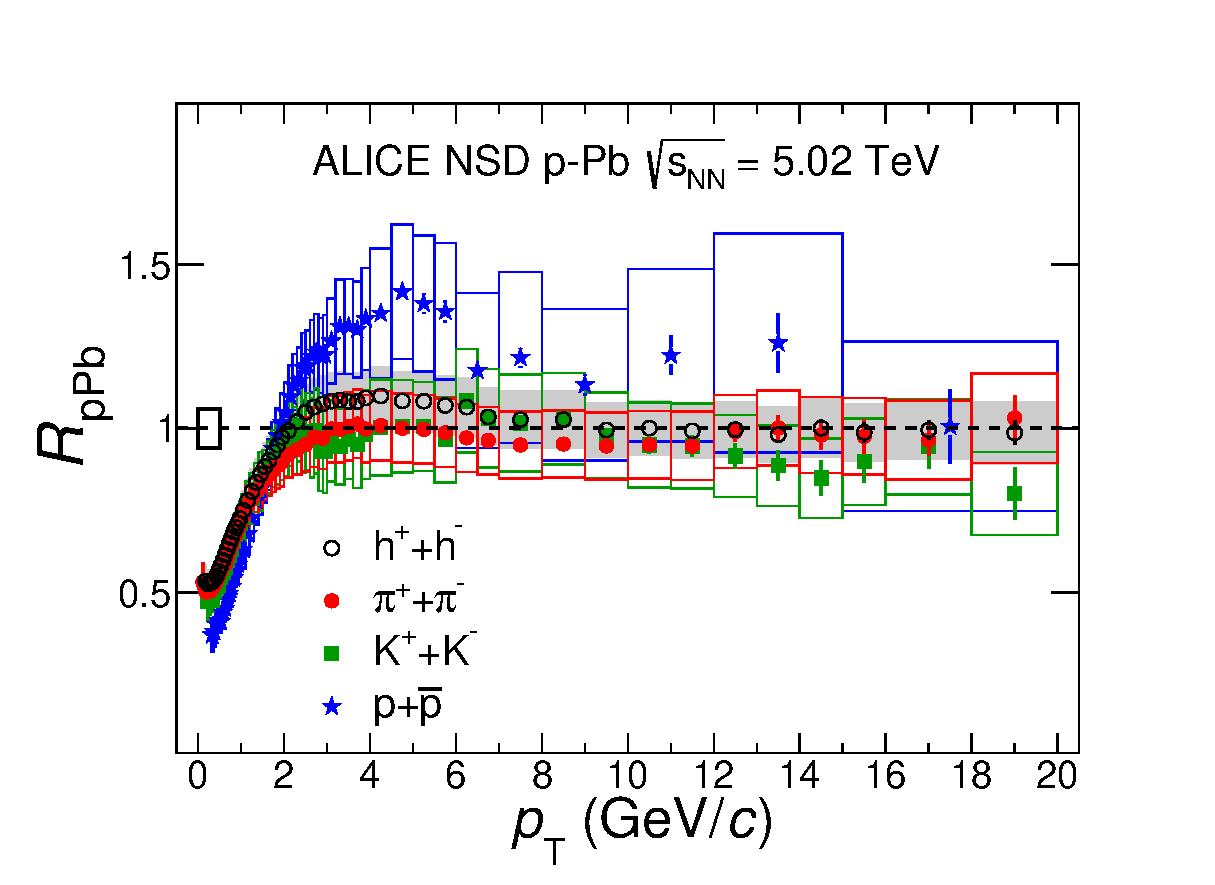
\includegraphics[width=10cm]{chap2/figure/Cronin/ChargeRpPb_ALICE.eps}
%  \caption{Inclusive $R_{pPb}$ of charged particles, $\pi$, K, $p$, $\Lambda$ at $\sqrt{s_{NN}}=$5.02 TeV~\cite{bib_chargerppb}.}
%  \label{fig_2_chargerppb}
%\end{figure}

%\begin{figure}[!h]
%  \begin{minipage}{0.5\hsize}
 %   \begin{center}
 %     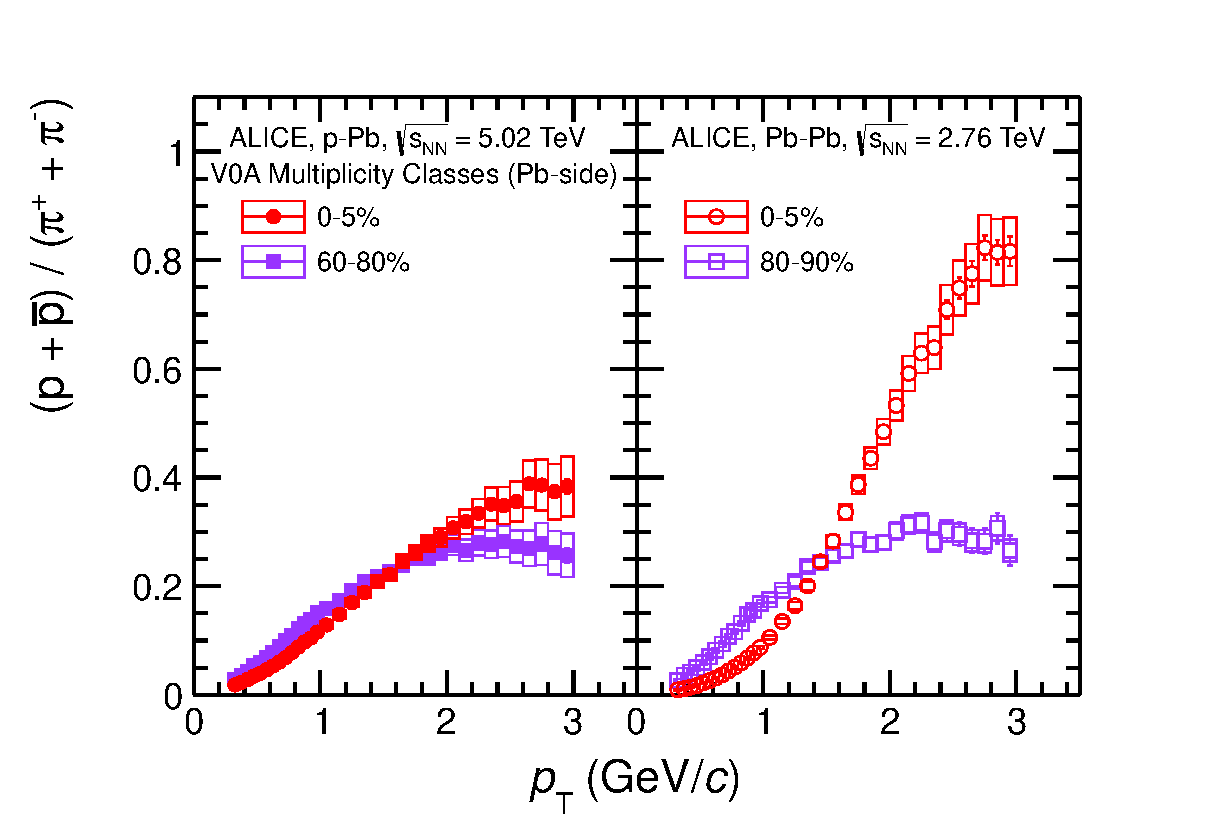
\includegraphics[width=8cm]{chap2/figure/Cronin/ProtonPionRatio_pPb.eps}
 %   \end{center}
 % \end{minipage}
 % \begin{minipage}{0.5\hsize}
 %   \begin{center}
 %     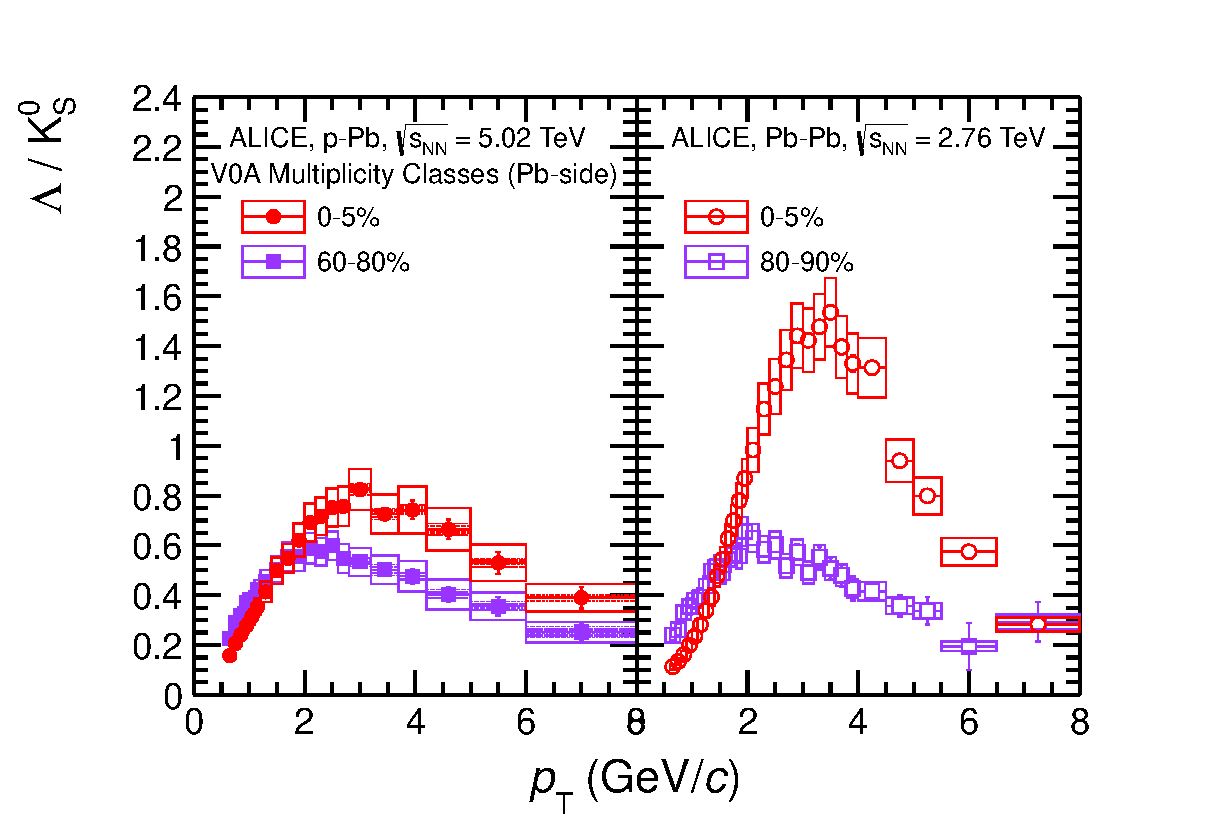
\includegraphics[width=8cm]{chap2/figure/Cronin/LambdaK0sRatio_pPb.eps}
 %   \end{center}
 % \end{minipage}
 % \caption{
 %   $p/\pi$ (Left) and $\Lambda$/$k^{0}_{s}$ (Right) ratio in p-Pb collisions at $\sqrt{s_{NN}}=$5.02 TeV~\cite{bib_alicebaryon}. 
 % }
 % \label{fig_2_baryonratio}
%\end{figure}




\subsection{Partonic Energy Loss inside the nucleus}
\label{sec_2_eloss}
Another initial state effect in heavy ion collisions is the initial state energy loss~\cite{bib_paeloss}. 
In the nuclear medium with the typical size $\sim L$, the medium induced radiative parton energy loss is expected due to the multiple interaction in the nucleus. 
%The average medium-induced radiative loss scaling as the quarkonium energy can be $\Delta E \sim E$.
%which corresponds to the time the scattered partons finish the radiative energy loss 
If the formation time of gluon radiation is shorter than the mean free path, the Cronin-like interaction mainly occurs and the radiation spectrum is similar to o the Bethe-Heitler spectrum, 
\begin{equation}
	\omega\frac{dI}{d\omega} = \frac{N_{c}\alpha_{s}}{\pi}\{  ln(1+\frac{\Delta q_{\rm{T}}^{2}E^{2}}{M_{\rm{T}}^{2} \omega^{2} }) -ln(1+\frac{\Lambda_{QCD}E^{2}}{M_{\rm{T}}^{2}\omega^{2}})    \}
\end{equation}
 where $E$ and $M_{\rm{T}}$ are the energy and transverse mass of the partons. 
 $\Delta q_{\rm{T}}$ is momentum transfer and $\Delta q_{\rm{T}}^{2}\sim\hat{q}L$ due to the momentum broadening in p-A collisions. 
$\hat{q}$ is called the transport coefficient.
In the limit of $\Lambda_{QCD} ^{2} \ll \Delta q_{\rm{T}}^{2} \ll M_{\rm{T}}^{2}$, the scaling of average energy loss $\Delta E \propto E$ is derived~\cite{bib_deltaescale}.       

When the formation time is longer than the mean free path, the coherent energy loss known as the Landau-Pomeranchuk-Migdal (LPM) effect occurs. 
In QED, this effect suppress medium induced bremsstrahlung radiation compared to the Bethe-Heitler process due to the interference between the next scatterings. 
The similar mechanism is expected in case of QCD process and the average energy loss is denoted by  $\Delta E_{\rm{LPM}} \propto \alpha_{s} \hat{q} L^{2}$.
This process can be expected in other nuclear matter effects like gluon shadowing. 

Furthermore, if the formation time is larger than path length $L$, the process is fully coherent and all scattering centers act as a source of radiation the coherent energy loss expressed by
\begin{equation}
	\Delta E \propto \alpha_{s}N_{c}\frac{\sqrt{\hat{q}L}}{M_{T}}E  ~ \gg \Delta E_{\rm{LPM}}
\end{equation}


\begin{figure}[!h]
    \begin{center}
      \includegraphics[width=12cm]{chap2/figure/eloss/eloss_arelo.png}
    \end{center}
  \caption{
  	Schematic of view of quarkonium hadroproduction in the nucleus rest frame~\cite{bib_jpsipaeloss}. 
  }
  \label{fig_2_jpsipaeloss}
\end{figure}

In case of $J/\psi$ production, the color nutralization time of the color octet state ($\tau_{octet}$) is expected larger than the perturbative time scale ($\tau_{hard}\sim 1/M$). 
Figure~\ref{fig_2_jpsipaeloss} shows the quarkonium hadroproduction in the nucleus rest frame~\cite{bib_jpsipaeloss}. 
In the nucleus mass frame, quarkonium hadroproduction by $gg\rightarrow Q\bar{Q}$ looks like small angle scattering of an color charge. 
The hadronization time ($t_{\psi} \gtrsim t_{octet} = \tau_{octet}(E/M)$) is expected long enough and hadronization happens outside of the nucleus.  
In this situation, the medium induced coherent spectrum arises from the interference between the gluon emission in the initial and final states.
The cross section of $J/\psi$ production in p-A collisions can be written by, 
\begin{equation}
	\frac{1}{A}\frac{d\sigma^{J/\psi}_{\rm{p}A}}{dE}(E, \sqrt{s})  = \int^{E}_{0}d\epsilon P (\epsilon ) \frac{d\sigma^{J/\psi}_{pp}}{dE}(E +\epsilon , \sqrt{s})
\end{equation}
where $P (\epsilon )$ is quenching weight related to the induced gluon spectrum and it includes the transport coefficient $\hat{q}$.
Figure~\ref{fig_2_paeloss} shows the initial energy loss calculation in p-Pb collisions at $\sqrt{s_{NN}}=$5 TeV by F.~Arleo $et$ $al$~\cite{bib_jpsipaeloss}. 
The transport coefficient $\hat{q}$ is taken by 
\begin{equation}
	\hat{q} (x) = \frac{4\pi^{2}\alpha_{s}N_{c}}{N_{c}^{2}-1}\rho xG(x) \sim q_{0}(\frac{10^{-2}}{x})^{0.3}
\end{equation}
$x$ dependence is considered from the HERA data described in Section~\ref{sec_2_pdf}. 
$q_{0}$ is the only free parameter in their calculation and and $q_{0} = 0.075 \rm{GeV}^{2}/$fm is obtained from the fit to E866 p-W collision data~\cite{bib_e866}.   
If the modification of Parton nPDF is neglected, the energy loss is expected to suppress the yield by a factor 20\%.

\begin{figure}[!h]
  %\begin{minipage}{0.5\hsize}
    %\begin{center}
  %\includegraphics[width=8cm]{chap2/figure/eloss/eloss_rhic.png}
    %\end{center}
  %\end{minipage}
  %\begin{minipage}{0.5\hsize}
    \begin{center}
      \includegraphics[width=8cm]{chap2/figure/eloss/eloss_lhc.png}
    \end{center}
  %\end{minipage}
  \caption{
    %Comparison of $J/\psi$ production between experimental data from RHIC and energy loss model calculation with various nPDF assumptions in d-Au\
% collision at $\sqrt{s_{NN}}=$200 GeV (Left) and Prediction of $J/\psi$ $R_{pPb}$ in p-Pb collision at $\sqrt{s_{NN}}=$ 5 TeV (Right)~\cite{bib_paeloss}.
    Prediction of $J/\psi$ $R_{pPb}$ in p-Pb collision at $\sqrt{s_{NN}}=$ 5 TeV by the energy loss model calculation with 4 nPDF settings~\cite{bib_paeloss}.
  }
  \label{fig_2_paeloss}
\end{figure}


\subsection{Nuclear Absorption}
$J/\psi$ produced at the initial parton scattering interacts with the nucleons in colliding nuclei and some fraction of $J/\psi$ decays into $D\bar{D}$. 
If the crossing time ($\tau_{c}$) of $c\bar{c}$ in the nuclear matter is longer than the formation time of quarkonia, quarkonia forms inside the nucleus and they interact the nucleons.
$\tau_{c}$ is calculated with, 
\begin{equation}
  \tau_{c} = \frac{L}{(\beta_{z}\gamma )}
\end{equation}
where  $\beta_{z}$ is longitudinal velocity of $c\bar{c}$. 
This effect describes the data at SPS energy well.
As Lorentz-$\gamma$ factor increases, the crossing time becomes short and quarkonium forms outside the nuclei. 
In this case, this absorption effect is negligible. 


The number of $J/\psi$ which interact and break up into $D\bar{D}$ is expressed by 
\begin{equation}
  L\rho_{0}\sigma_{abs}
\end{equation}
where $L$ is the effective path length, $\rho$ is the normal nuclear density, and $\sigma_{abs}$ is the absorption length. 
$L$ is calculated in Glauber model as following with the impact parameter\bm{b}, 
\begin{equation}
  L = \frac{1}{\rho_{0}}\frac{\int T_{A}(\bm{s})  T_{B}(\bm{b}-\bm{s}){A-1}T_{A}(\bm{s})+(B-1)T_{B}(\bm{b}-\bm{s}) d\bm{s} }
  {
    s\int T_{A}(\bm{s})T_{B}(\bm{b}-\bm{s})d\bm{s}    
  }
\end{equation}
The cross section of $J/\psi$in p-$A$ collisions is expressed as, 
\begin{equation}
	\sigma_{J/\psi , \rm{p}A} = \sigma_{J/\psi, pp}Ae^{-\rho_{0} L}\sigma_{abs}
\end{equation}

Figure~\ref{fig_2_sigmaabs} shows the measured $\sigma_{abs}$ as a function of collision energies\cite{bib_crosstime}. 
As collision energy increases, $\sigma_{abs}$ decrease due to the large $\gamma$ factor. 
\begin{figure}[!h]
  \begin{center}
    \includegraphics[width=8cm]{chap2/figure/experimentaldata/sigmaabs.png}
  \end{center}
  \caption{
    Measured $\sigma_{abs}$ at $y=0$ as a function of collision energy~\cite{bib_crosstime}. }
  \label{fig_2_sigmaabs}
\end{figure}



\section{Previous Measurements of $J/\psi$ production}
%$R_{AA}$ of $J/\psi$ 
%Figure~\ref{} shows the measurement of $J/\psi$ anisotropic flow with respective to the event plane. 
%The non-zero v2 suggest the regeneration of $J/\psi$




\subsection{SPS Results}
$J/\psi$ has been measured at the Super Proton Synchrotron (SPS) in CERN in S-U, Pb-Pb, and In-In collisions at $\sqrt{s_{NN}}~=$ 19.4, 17.3, and 17.3 GeV, respectively. 
The collision system and energy of charmonium experiments at SPS is summarized in Table.~\ref{table_2_sps}

\begin{table}
\centering 	
	\begin{tabular}{cccc} \\ \hline
	Experiment  & System                        &      $\sqrt{s_{NN}$ & Reference \\ \hline
	NA38            & p-Cu, U, W                 &   19.4                     & \cite{bib_2_na38pal1,bib_2_na38pal2,bib_2_na38pal3,bib_2_na38pal4}     \\
	~                   & p-, C, Al, Cu, W           & 29.1                     & \cite{bib_2_na38pah}    \\
	~                   & O-U, O-Cu, O-U,S-U   & 19.4                      & \cite{bib_2_na38aa1,bib_2_na38aa2,bib_2_na38aa3,bib_2_na38aa4,bib_2_na38aa5}   \\
	NA50           & p-Be, Al, Cu, Ag, W      &          27.4            & \cite{bib_2_na50pa1,bib_2_na50pa2} \\
	       ~             & Pb-Pb                           &    17.3                 & \cite{bib_2_na50aa1,bib_2_na50aa2,bib_2_na50aa3,bib_2_na50aa4,bib_2_na50aa5,bib_2_na50aa6,bib_2_na50aa7} \\ 
%	NA60           & p-Be,Al, Cu, In, W, Pb, U  & 
	NA60           &  In-In                             & 17.3                    &  \cite{bib_2_na60aa}  \\ \hline
	\end{tabular}		
	\caption{The collision system and energy of charmonium experiments at SPS.}
	\label{table_2_sps}
\end{table}

\end{table}
Figure~\ref{fig_2_ratiodrell} shows the ratio of measured yields to the Drell-Yang process as a function of path length in p-$A$ and $A$-$A$ collisions at NA38, NA50, NA51 since the yields of Drell-Yang process is scaled by the number of binary nucleon-nucleon collisions ($\langle N_{coll}\rangle$) described in Appendix.~A~\cite{bib_2_na50aa6} . 
p-$A$ results show the common trend due to the normal nuclear matter effects. 
From this dependence, the nuclear absorption cross section $\sigma_{abs}$ of $J/\psi$ was determined to be $\sigma_{abs}~=$ 4.2 $\pm$ 0.5 mb. 
%The solid curve shows the expected ratio including nuclear absorption. 
Figure~\ref{fig_2_ratiodrell} shows the ratio of measured cross section of $J/\psi$ and the expected yield from the normal nuclear matter effects as a function of path length $L$ in Pb-Pb collisions at $\sqrt{s_{NN}}~=$ 17.3 and 19.4 GeV at NA38, and NA50, respectively~\cite{bib_2_na50aa7}. 
The results show the clear suppression as $L$ increases in particular less bound state $\psi$. 
%The nucleus crossing time ($\tau_{c}\sim$ 0.3 fm/c) is compatible or larger than the charmonium formation time.
%At large path length, stronger suppression is observed than the normal nuclear matter effects. 
%\begin{figure}[!h]
%  \centering
%  \includegraphics[width=10cm]{chap2/figure/experimentaldata/sps_cnm.png}
%  \caption{The ratio of the measured $J/\psi$ yield to Drell-Yang process  as a function of path length in p-A and A-A collisions at NA38, NA50 and NA51\cite{bib_na50}.}
%  \label{fig_2_na50_1}
%\end{figure}
%\begin{figure}[!h]
%  \centering
%  \includegraphics[width=10cm]{chap2/figure/experimentaldata/Jpsi_SPS_HIC.png}
%  \caption{The ratio of the measured yield to the expected yield of $J/\psi$ and $\psi^{'}$ as a function of path length in A-A collisions at NA38, NA50 and NA51\cite{bib_na50}.}
%  \label{fig_2_na50_2}
%\end{figure}
\begin{figure}[!h]
  \begin{minipage}{0.5\hsize}
    \begin{center}
      \includegraphics[width=8cm]{chap2/figure/experimentaldata/sps_cnm.png}
    \end{center}
  \end{minipage}
  \begin{minipage}{0.5\hsize}
    \begin{center}
      \includegraphics[width=8cm]{chap2/figure/experimentaldata/Jpsi_SPS_HIC.png}
    \end{center}
  \end{minipage}
  \caption{
	The ratio of the measured $J/\psi$ yields to Drell-Yang process  as a function of path length in p-$A$ and $A$-$A$ collisions at NA38, NA50 and NA51 (Left)  and the ratio of the measured yields to the expected yields of $J/\psi$ and $\psi^{'}$ as a function of path length in A-A collisions at NA38, NA50 and NA5\cite{bib_2_na50aa6,bib_2_na50aa7}.
	}
  \label{fig_2_ratiodrell}
\end{figure}
Figure~\ref{fig_2_inin} shows the ratio of measured yield to the expected yield in In-In collisions at NA60 and Pb-Pb collisions at NA50 at $\sqrt{s_{NN}}~=$ 17.3 GeV as a function of $N_{part}$ described in Appendix A~\cite{bib_2_na60aa}. 
In high $N_{part}$ (centrality) events, significant suppression is observed in both Pb-Pb and In-In collisions above $N_{part}~>$ 80. 
\begin{figure}[!h]
  \centering
  \includegraphics[width=10cm]{chap2/figure/experimentaldata/sps_ininpbpb.png}
  \caption{The ratio of the measured yields to expected yields from the normal nuclear matter effects as a function of $N_{part}$ in Pb-Pb and In-In collisions\cite{bib_2_na60aa}. }
  \label{fig_2_inin}
\end{figure}

Figure~\ref{fig_2_spsmeanpt} shows the path length dependence of mean squared transverse momentum  $\langle p_{\rm{T}}^{2}\rangle$\cite{bib_2_na50aa4}. 
$\langle p_{\rm{T}}^{2}\rangle$ increases with mass number $A$ that is similar trend to Cronin effect. 
The results are fitted using the Cronin parametrization and $a_{gN} = $0.081 $\pm$ 0.004 and 0.078 $\pm$ 0.006 at $\sqrt{s_{NN}} = $ 17.3 and 19.4 GeV, respectively. Similar slope values are obtained. 
%Further measurements at HERAB and FNAL, it is indicated the slope of Cronin parametrization is independent of collision energy. 
\begin{figure}[!h]
  \centering
  \includegraphics[width=10cm]{chap2/figure/experimentaldata/sps_meanpt.png}
  \caption{The mean squared transverse momentum $\langle p_{\rm{T}}^{2}\rangle$ of $J/\psi$ in p-$A$ and $A$-$A$ collisions~\cite{bib_2_na50aa4}. }
  \label{fig_2_spsmeanpt}
\end{figure}

\subsection{E866 at Tevatron}
E866 at Tevatron in Felmi National Accelerator Laboratory (FNAL) has a wide Feynmann $x$ coverage at -0.1 $<$ $x_{F}$ $<$ 0.93. 
Feynmann-$x$ is defined as the longitudinal momentum transfer fraction $x_{1}$ and $x_{2}$ in the the projectile and the target, respectively, 
\begin{equation}
  x_{F}  = x_{1}-x_{2}
\end{equation}
%where $p_{L}$ is the longitudinal momentum. 
E866 evaluates the nuclear matter effects with parameter $\alpha$ defined as, 
\begin{equation}
  \sigma^{J/\psi}_{AB} = \sigma^{J/\psi}_{NN}(AB)^{\alpha}
\end{equation}
where $A$ and $B$ are the mass number of colliding nuclei. 
$\sigma^{J/\psi}_{AB}$ is the $J/\psi$ cross section in $A$-$B$ collisions and $\sigma^{J/\psi}_{NN}$ is the $J/\psi$ cross section in nucleon-nucleon collisions. 
Figure~\ref{fig_2_e866} shows the measured $\alpha$ as a function of $x_{F}$ in p-$A$ (p-Fe, p-W) collisions at $\sqrt{s_{NN}}~=$ 38.8 GeV. 
E866 observed $J/\psi$ suppression at high $x_{F}$ region in p-Fe and p-W collisions at $\sqrt{s_{NN}}~=$ 38.8 GeV, while  $\alpha $ is saturated to 0.96 $\pm$ 0.01 at low $x_{F}$. 
%At low $x_{F}$, quarkonium forms inside the nucleus. 
%One possibility to describe the suppression at high $x_{F}$ is a partonic interaction inside the nucleus since charmonium is expected to form outside the nucleus at high $x_{F}$ limit~\cite{bib_paeloss}.  
\begin{figure}
  \centering
  \includegraphics[width=8cm]{chap2/figure/experimentaldata/e866_xf.png}
  \caption{ $x_{F}$ dependence of $\lpha$ on $J/\psi$ production for three different data set (Top) and  $x_{F}$ and comparison between $J/\psi$ and $\psi$ (Bottom) at $\sqrt{s_{NN}}~ =$ 38.8 GeV~\cite{bib_e866}. }
  \label{fig_2_e866}
\end{figure}

\subsection{RHIC}
\label{rhic}
\subsubsection{d-Au Collisions}
\label{sec_2_dau}
\begin{figure}[!h]
  \begin{minipage}{0.5\hsize}
    \begin{center}
      \includegraphics[width=8cm]{chap2/figure/experimentaldata/jpsi_phenixdAu.png}
    \end{center}
  \end{minipage}
  \begin{minipage}{0.5\hsize}
    \begin{center}
      \includegraphics[width=8cm]{chap2/figure/eloss/eloss_rhic.png}
    \end{center}
  \end{minipage}
  \caption{
    $J/\psi$ production in d-Au at $\sqrt{s_{NN}}=$200 GeV/c measured by PHENIX at RHIC and model comparison with the NLO calculation with EPS09 nPDF and gluon saturation model (Left) Comparison of $J/\psi$ production between experimental data from RHIC and energy loss model calculation with various nPDF assumptions in d-Au collisions at $\sqrt{s_{NN}}=$200 GeV (Right)~\cite{bib_rhicjpsirdauvsy,bib_rhicjpsirdauvspt}. 
  }
  \label{fig_2_jpsiparhic}
\end{figure}
The left panel of Fig.~\ref{fig_2_jpsiparhic} shows the comparison of $J/\psi$ production between the measured results and the calculation based on the nuclear shadowing and the gluon saturation  at $\sqrt{s_{NN}}=$200 GeV~\cite{bib_rhicjpsirdauvsy}. 
The results show the suppression of $J/\psi$ production in whole measured  rapidity region. 
Shadowing $+$ hadron break up model describes $y$ dependence.
%However the $p_{T}$ dependence of $R_{\rm{dAu}}$. 
The right panel of Fig.~\ref{fig_2_jpsiparhic} shows the comparison of $J/\psi$ production between experimental data from RHIC and energy loss model calculation with various nPDF assumptions in d+Au collision at $\sqrt{s_{NN}}=$200 GeV~\cite{bib_jpsipaeloss}. 
The model shows the nPDF depedence in particular considering EPS09 PDF especially backward. 
It is thought the difference of strength of the anti-shadowing region ($x\sim ~10^{-1}$) as shown in Fig.~\ref{fig_2_pdf}.
Within the uncertainty of the nPDF, the energy loss model shows the reasonable agreement at mid-rapidity and forward rapidity. 
The mechanism of normal nuclear matter effects in d+Au collisions at RHIC is still  under discussion. 

\subsubsection{Heavy Ion collisions}
\begin{figure}[!h]
  \centering
  \includegraphics[width=10cm]{chap2/figure/experimentaldata/rhicjpsiaa.png}
  \caption{$N_{part}$ dependence of the nuclear modification factor of $J/\psi$ at mid-rapidity and forward rapidity (Upper) and the ratio of the nuclear modification factor of $J/\psi$ between forward rapidity and mid-rapidity~\cite{bib_rhicjpsiraa}.}
  \label{fig_2_rhicjpsiaa}
\end{figure}
Figure~\ref{fig_2_rhicjpsiaa} shows the nuclear modification factor of $J/\psi$ at mid-rapidity and forward rapidity in Au-Au collisions at $\sqrt{s_{NN}}=$200 GeV~\cite{bib_rhicjpsiraa}. 
The results show the strong suppression of $J/\psi$ in Au-Au collisions at both mid-rapidity and forward rapidity. 
The lower panel of Fig.~\ref{fig_2_rhicjpsiaa} shows the ratio of forward/mid nuclear modification factor.  
At $N_{part} > $100, the $J/\psi$ production at forward rapidity is also suppressed in Au-Au collisions. 
%It looks inconsistent with the color screening picture because the energy density at mid-rapidity is expected higher than that at forward rapidity. 
%This result may suggest the existence of $J/\psi$ regeneration at RHIC. 
As discussed in Section~\ref{sec_2_dau}, the measured $R_{AA}$ is affected by non-negligible normal nuclear matter effects.
In addition to the difference of the probing temperature,  the discrepancy of the results between mid-rapidity and forward rapidity is expected to come from the normal nuclear matter effects. 

In order to estimate the contribution of the normal nuclear matter effect in $J/\psi$ $R_{AA}$ experimentally, d-Au data is used and they assumes the $R_{AA}$ can be treated as a convolution of p-Au collisions~\cite{bib_daucorr,bib_daucorr2}. 
The rapidity dependent absorption cross section $\sigma^{J/\psi}_{abs}$ is extracted by fitting of EKS98 and nDSg shadowing parametrization as shown in the left panel of Fig.~\ref{fig_2_cnmraa}~\cite{bib_daucorr2}. 
The large global uncertainties come from the uncertainty of Glauber estimation of $N_{coll}$ in d-Au collisions. 
Since there is a significant difference between the impact parameter dependence of $R_{\rm{pAu}}$ and $R_{\rm{dAu}}$ mainly due to the smearing caused by the finite size of the deuteron, $R_{\rm{pAu}}$ is calculated using EKS98 and nDSg shadowing parametrization obtained by fitting to d-Au data~\cite{bib_shadowmodel}. 

The normal nuclear matter $R_{AA}$ is estimated by the Glauber calculation of Au-Au collisisions using the fitted absorption cross sections and the centrality dependent $R_{\rm{pAu}}$. 
For each nucleon-nucleon collisions, impact parameter $b_{1}$ and $b_{2}$ are determined with respect to each target nucleus and then $R_{\rm{pAu}}(b_{1}, y) \times R_{\rm{pAu}}(b_{2}, -y)$ is calculated and added to the accumulated $R_{AA}$. 
After processing all events, the accumulated $R_{AA}$ is divided by the number of events. 
The right panel of Fig.~\ref{fig_2_cnmraa} shows the estimated normal nuclear matter $R_{AA}$ in Au-Au collisions at $\sqrt{s_{NN}} =$ 200 GeV.
Although the absorption cross section has large global uncertainties due to the uncertainty of $N_{coll}$, it can be compensated and then negligible in the calculation of the normal nuclear matter $R_{AA}$  
The kinematic dependent difference in the absorption cross section do not affect the normal nuclear matter $R_{AA}$. 
As long as the method of fitting the d-Au data is consistent with the estimate of the normal nuclear matter $R_{AA}$ , the result should  be model independent. 

\begin{figure}[!h]
  \begin{minipage}{0.5\hsize}
    \begin{center}
      \includegraphics[width=8cm]{chap2/figure/experimentaldata/phenix_absxsection.png}
    \end{center}
  \end{minipage}
  \begin{minipage}{0.5\hsize}
    \begin{center}
      \includegraphics[width=8cm]{chap2/figure/experimentaldata/phenix_cnmraa.png}
    \end{center}
  \end{minipage}
  \caption{
  	Rapidity dependent absorption cross section in d+Au collisions at $\sqrt{s_{NN}}=$200 GeV(Left) and normal nuclear matter $R_{AA}$ in Au-Au collisions estimated from d-Au data at $\sqrt{s_{NN}}=$200 GeV with EKS98 parametrization (Right)~\cite{bib_daucorr2}. 
  }
  \label{fig_2_cnmraa}
\end{figure}

%To correct the nuclear matter effects, the survival fraction is defined as the ratio of $R_{AA}$ to the expected modification from the normal nuclear matter effects.
%The expected yield is extracted from the experimental data or realistic model calculation. 
%PHENIX corrected the normal nuclear matter effects using the measured d-Au results~\cite{bib_daucorr}.  
Figure~\ref{fig_2_saavse} shows $S_{AA}$ which is defined by $R_{AA}$ divided by the normal nuclear matter $R_{AA}$ as a function of the initial energy density $\epsilon _{0}$ and the formation time $\tau_{0}$for RHIC and SPS data~\cite{bib_rhicjpsisaa}.
\begin{figure}[!h]
  \centering
  \includegraphics[width=10cm]{chap2/figure/experimentaldata/saa.png}
  \caption{Survival fraction ($S_{AA}$) of the RHIC and SPS data as a function of $\tau_{0}  \epsilon_{0}$~\cite{bib_rhicjpsisaa}. }
  \label{fig_2_saavse}
\end{figure}
%In this case, formation time $\tau_{0}$ is taken as 1 fm/$c$ for all data. 
After consideration of the normal nuclear matter effects, the both results of forward and mid-rapidity shows the same monotonic suppression as a function of $\epsilon \tau$. 
Furthermore hydro$+$ $J/\psi$  model calculation describes the PHENIX data well the melting temperature $=$ 2$T_{c}$ as shown in the left panel of Fig.~\ref{fig_2_lhc_gunjicalc}~\cite{bib_gunjicalc}. 
The understanding and determination of the normal nuclear matter from the measured d-Au results allows this quantitative model comparison. 
However, regeneration calculation also show the reasonable agreement to the experimental results as shown in the right panel~\cite{bib_recomodel}. 
The mechanism of $J/\psi$ production in heavy ion is still under discussion and the LHC measurements play a crucial role on this problem. 
%both of RHIC and SPS data shows the same trend of the initial energy density dependence. 
%As another investigation of normal nuclear matter effects,  asymmetric Cu+Au collision. 
%Due to the difference of nPDF in Au and Cu, 
\begin{figure}[!h]
  \begin{minipage}{0.5\hsize}s
    \begin{center}
      \includegraphics[width=8cm]{chap2/figure/experimentaldata/gunjicalc.png}
    \end{center}
  \end{minipage}
  \begin{minipage}{0.5\hsize}
    \begin{center}
      \includegraphics[width=8cm]{chap2/figure/experimentaldata/pbmreco.png}
    \end{center}
  \end{minipage}
  \caption{
	Comparison of the PHENIX results and the hydrodynamic calculation including the  melting effects of quarkonium (Left) and the statistical regeneration model~\cite{bib_gunjicalc,bib_recomodel}.
   }
  \label{fig_2_lhc_gunjicalc}
\end{figure}



\subsection{LHC measurements}
Since the collision energy of LHC is higher than RHIC,  stronger suppression due to the color screening is expected. 
%The left panel of Fig.~\ref{fig_2_lhc_raavsnpart} shows the $J/\psi$ $R_{AA}$ in Pb-Pb collisions at $\sqrt{s_{NN}}~=$ 2.76 TeV at forward rapidity~\cite{bib_alicejpsiraa}. 
%The result shows less suppression compared with the RHIC results. 
\begin{figure}[!h]
	\centering
	  \includegraphics[width=15cm]{chap2/figure/experimentaldata/jpsiraa_npart.png}
 	 \caption{ $J/\psi$ $R_{AA}$ as a function of the charged particle multiplicity at mid-rapidity (Left) and forward rapidity (Right) in Pb-Pb collisions at $\sqrt{s_{NN}}~=$ 2.76 TeV and Au-Au $\sqrt{s_{NN}}~=$ 200 GeV~\cite{bib_anton}. }
  \label{fig_2_raanpart}
\end{figure}
%The right panel of Fig.~\ref{fig_2_lhc_raavsnpart} shows the $J/\psi$ $R_{AA}$ as a function of $p_{\rm{T}}$ and the comparison to the RHIC results and model calculations at mid-rapidity~\cite{bib_alicejpsiraamid}. 
Figures~\ref{fig_2_raanpart} show the measured $J/\psi$ $R_{AA}$ as a function of the charged particle multiplicity at mid-rapidity and forward rapidity at RHIC and LHC~\cite{bib_anton}.
Less suppression at LHC was observed  at both mid-rapidity and forward rapidity. 
The discrepancy of RHIC and LHC results might be related to the $J/\psi$ regeneration. 
On the other hand, the modification of the normal nuclear matter effects is different between RHIC and LHC. 
And thus the investigation of the normal nuclear matter effects at LHC is crucial to understand the energy dependence of $J/\psi$ production. 
At mid-rapidity in ALICE, the results show no multiplicity dependence. 
The high multiplicity events correspond to high initial energy density events. 
Therefore a simple color screening picture cannot explain this dependence. 
This result also the recombination picture. 

Figures~\ref{fig_2_raapt} show the measured $J/\psi$ $R_{AA}$ as a function of $p_{\rm{T}}$ at mid-rapidity and forward rapidity at RHIC and LHC~\cite{bib_alicejpsiraa,bib_alicejpsiraamid}.
At higher $p_{\rm{T}}$, $R_{AA}$ is compatible to the RHIC result. 
On the other hand, a large enhancement is observed above 4 GeV/$c$.
The $J/\psi$ regeneration picture gives a reasonable explanation to this enhancement. 
The transport model calculation shows the agreement to the ALICE result. 
This model calculation considers the all collision stages including both the color screening and $J/\psi$ regeneration. 
\begin{figure}[!h]
  \begin{minipage}{0.5\hsize}
  \begin{center}
	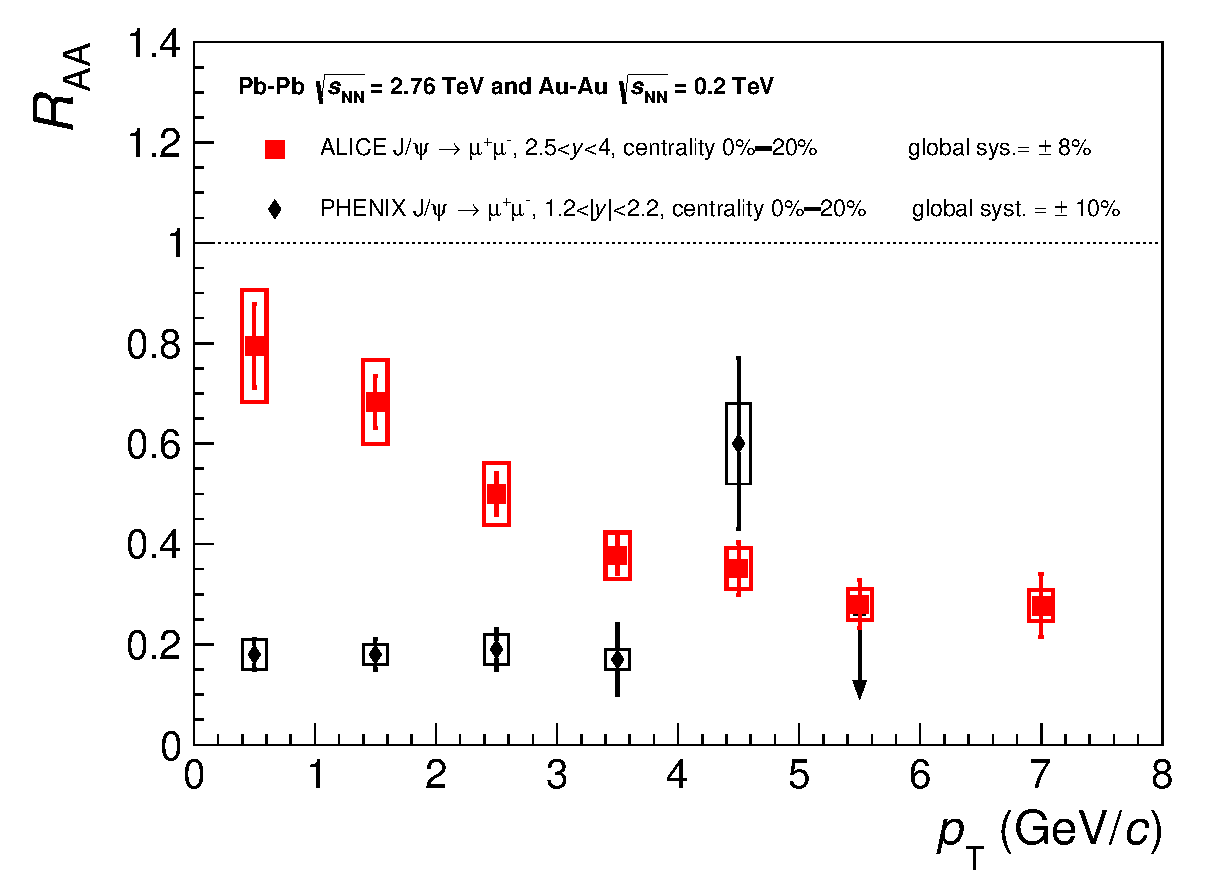
\includegraphics[width=8cm]{chap2/figure/experimentaldata/RAAPtvsModels2-4514.eps}	  
    \end{center}
  \end{minipage}
  \begin{minipage}{0.5\hsize}
   \begin{center}
      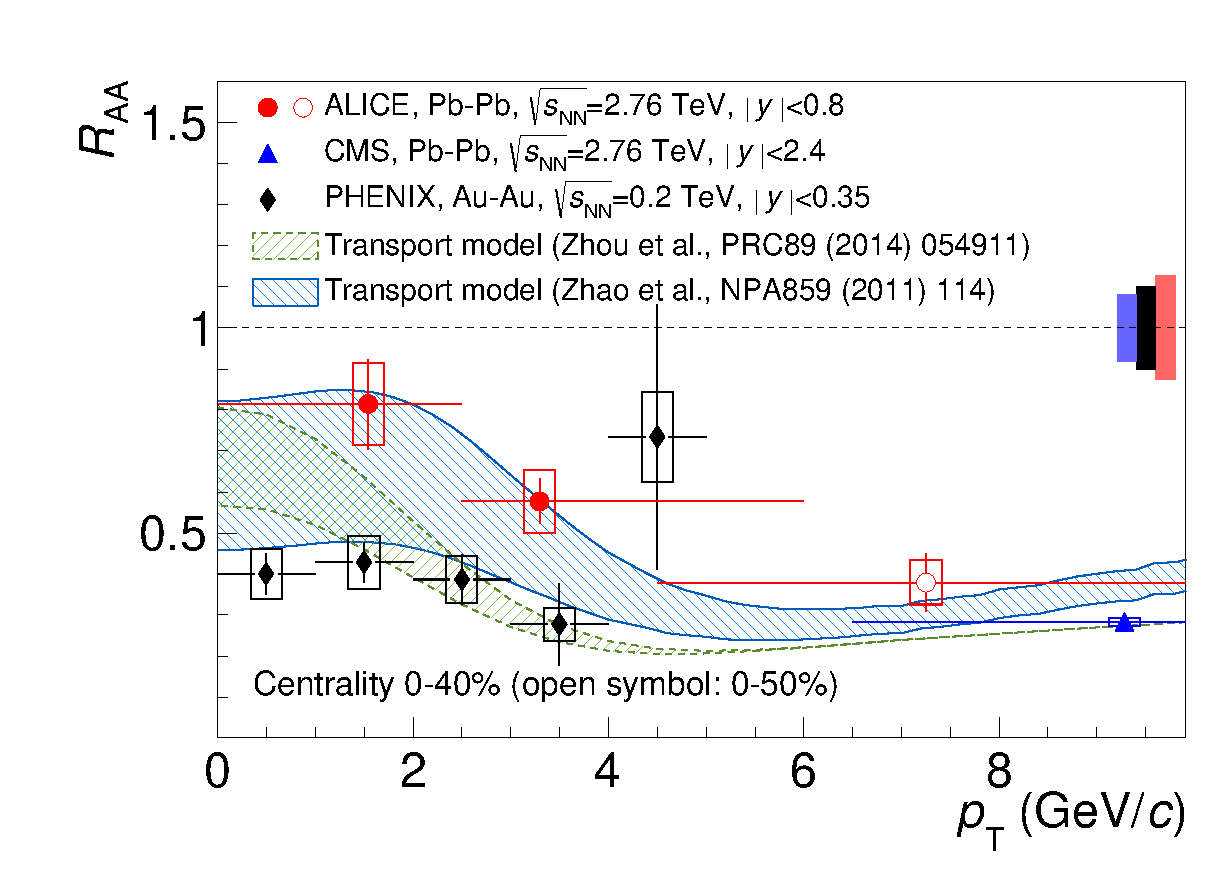
\includegraphics[width=8cm]{chap2/figure/experimentaldata/Raa-Mpt-sysBar-compPHENIX-compCMS-tcompZhou-tcompZhao-13709.eps}
    \end{center}
  \end{minipage}
  \caption{
	$J/\psi$ $R_{AA}$ as a function of the charged particle multiplicity at mid-rapidity (Left) and forward rapidity (Right) in Pb-Pb collisions at $\sqrt{s_{NN}}~=$ 2.76 TeV and Au-Au $\sqrt{s_{NN}}~=$ 200 GeV~\cite{bib_alicejpsiraa,bib_alicejpsiraamid}.
   }
  \label{fig_2_raapt}
\end{figure}

\section{Normal Nuclear Matter Effects at LHC}
Due to the large $\gamma$ factor at LHC, short crossing time of $c\bar{c}$ in the nuclear matter is expected $\sim$ $10^{-2}$ fm/$c$.
Therefore the nuclear absorption might be small or negligible at LHC energy.
The modification of nPDF is expected more crucial since more compared to the RHIC results smaller $x$ is probed at $10^{-4}$-$10^{-3}$.  
At forward or low $p_{\rm{T}}$ measurement is expected to show up the gluon saturation effect.
Cronin effect is also expected to show up in LHC measurements. 
The model calculation of the initial state energy loss in nucleus predicts relevant modifications of the $J/\psi$ production in p-Pb collisions. 

However the mechanism of normal nuclear matter is still unknown and theoretical calculations have finite uncertainties. 
%Due to the less sensitivity of Deep Inelastic Scattering, gluon nPDF still has large uncertainty at small $x$ region as described in Section.~\ref{sec_2_pdf}. 
In order to understand the normal nuclear matter effects with high precision, the experimental results of p-$A$ collisions are crucial. 
The motivation of this thesis is the investigation of normal nuclear matter effects in p-Pb collisions experimentally. 
To discuss normal nuclear matter effects, the nuclear modification factor is useful, 
\begin{equation}
  R_{\rm{pPb}} = \cfrac{Y_{\rm{pPb}}}{\langle N_{coll}\rangle Y_{\rm{pp}}}
\end{equation}
where $\langle N_{coll} \rangle$ is the average number of binary nucleon-nucleon collisions in p-Pb collisions and $Y_{\rm{pPb}}$ and $Y_{\rm{pp}}$ are yield of $J/\psi$ in p-Pb and pp collisions. 
The discrepancy from unity of $R_{\rm{pPb}}$ means the indication of nuclear matter effects. 
Normal nuclear matter effects described in this chapter are sensitive $x$, $Q$, and path length. 
Therefore the systematic measurements for the collision energy, rapidity, $p_{\rm{T}}$, and the impact parameter dependence provides  key information to understand the nuclear matter effects. 

%\section{Motivation of this study}
%The motivation of this thesis is the determine the magnitude of normal nuclear matter effects experimentally to extract the QGP signals from the result of heavy ion collisions. 
%From measured $R_{pPb}$, the extraction of $S_{AA}$ is useful for a direct comparison to $R_{AA}$. 
%The normal nuclear matter effects in heavy ion collisions is factorized by the square of the nuclear modification factor in p-Pb collisions $R_{\rm{pPb}}$ 
%\begin{equation}
%	S_{AA} ~= ~ \frac{R_{AA}}{(R_{\rm{pPb}})^{2}}
%\end{equation}
%The comparison ofof and see the initial energy dependence is important to study the thermodynamics of the system as . 

